\chapter{Project Requirements}

This chapter provides a comprehensive specification of the functional and non-functional requirements for the complete MyAIStorybook system. The requirements are organized to reflect the modular architecture and user interactions supported by the platform implementation, encompassing foundational story generation capabilities through advanced interactive features.

\clearpage

\section{Use-case Analysis}

The MyAIStorybook platform supports comprehensive operational workflows encompassing story generation, interactive features, and advanced user engagement capabilities. The use case diagram illustrates the primary interactions between users and system functionalities.

\begin{figure}[H]
    \centering
    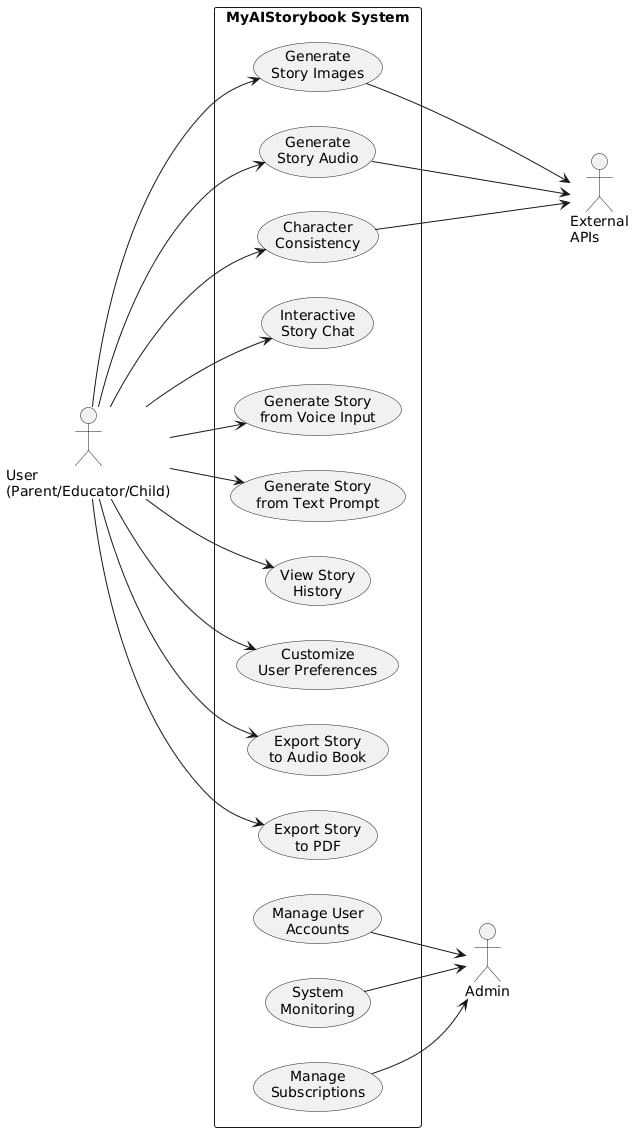
\includegraphics[width=0.75\textwidth]{diagram_images/use_case_diagram.jpg}
    \caption{Use Case Diagram illustrating interactions between users and system functionalities}
    \label{fig:usecase}
\end{figure}

The system supports seven primary use cases, each addressing specific user needs and interaction patterns. These use cases represent the core functionalities that users engage with throughout their journey from story ideation to final content consumption.

\textbf{UC1: Generate Story from Prompt} - Users input text prompts to generate complete illustrated storybooks through the multi-agent pipeline.

\textbf{UC2: Generate Story from Voice Input} - Users speak story prompts using voice input, which are transcribed and processed for story generation.

\textbf{UC3: Interactive Story Chat} - Users engage in conversational AI interactions to refine story requirements and receive personalized recommendations.

\textbf{UC4: Generate Story Images with Character Consistency} - The system creates high-quality illustrations maintaining consistent character appearance across all scenes.

\textbf{UC5: Generate Story Audio Narration} - Text-to-speech synthesis produces natural narration with emotion detection and character-specific voices.

\textbf{UC6: Export Story to PDF} - Complete stories are exported as professionally formatted PDF documents for printing and distribution.

\textbf{UC7: Export Story to Audio Files} - Audio narration is compiled into downloadable audio book formats with chapter markers.

\section{Functional Requirements}

This section details the specific functional capabilities required from each module of the MyAIStorybook system.

\subsection{Multi-Agent Story Generation Module}

\begin{enumerate}
    \item FR1.1: The system shall accept user prompts ranging from 5 to 500 characters for story generation
    \item FR1.2: The Prompt Agent shall validate user input and classify prompts as normal, detailed, invalid, or nonsense
    \item FR1.3: The Prompt Agent shall enhance simple prompts by adding contextual details while preserving user intent
    \item FR1.4: The Director Agent shall orchestrate the sequential execution of Writer, Reviewer, and Editor agents
    \item FR1.5: The Writer Agent shall generate structured stories with title, setting, characters, and scenes using Ollama LLM (llama3.1:8b-instruct-q4\_K\_M)
    \item FR1.6: The Writer Agent shall create exactly 3 scenes per story in the current implementation
    \item FR1.7: The Writer Agent shall retry up to 2 times if JSON parsing fails
    \item FR1.8: The Writer Agent shall develop character backstories and personality traits
    \item FR1.9: The Writer Agent shall generate dialogue and character interactions
    \item FR1.10: The Reviewer Agent shall validate generated content for coherence, age-appropriateness, and narrative consistency
    \item FR1.11: The Reviewer Agent shall assess educational value and learning objectives
    \item FR1.12: The Editor Agent shall refine story text, improve language quality, and ensure proper formatting
    \item FR1.13: The Editor Agent shall generate PDF export automatically during the editing phase
    \item FR1.14: The Evaluation Agent shall run in background to collect quality metrics without blocking the main response
    \item FR1.15: The system shall output stories in comprehensive JSON format with metadata and media paths
    \item FR1.16: The system shall save intermediate outputs from each agent in dedicated directories
    \item FR1.17: The system shall maintain processing status and emit console logs at each pipeline stage
    \item FR1.18: The system shall handle errors gracefully and return informative status messages
    \item FR1.19: The system shall learn from user preferences and adapt content generation accordingly
\end{enumerate}

\subsection{Image Generation Module}

\begin{enumerate}
    \item FR2.1: The Image Agent shall generate illustrations for each story scene using Stable Diffusion 1.5 with Realistic Vision checkpoint
    \item FR2.2: The system shall employ a two-pass generation process: txt2img synthesis followed by img2img high-resolution refinement
    \item FR2.3: The system shall truncate image prompts to 77 tokens or fewer to ensure CLIP model compatibility
    \item FR2.4: The Image Agent shall utilize DPMSolver scheduler with Karras sigmas for optimized sampling
    \item FR2.5: The system shall use GPU acceleration with half-precision (float16) when CUDA is available
    \item FR2.6: The system shall automatically fall back to CPU processing if GPU is unavailable
    \item FR2.7: The system shall save generated images in PNG format with unique, timestamped filenames
    \item FR2.8: The system shall organize images in the generated/images directory
    \item FR2.9: The Image Agent shall apply positive and negative prompts for quality control
    \item FR2.10: The system shall continue story generation even if image generation fails (graceful degradation)
    \item FR2.11: The system shall return image file paths in the story JSON for frontend access
    \item FR2.12: The system shall support optional image generation via user toggle
\end{enumerate}

\subsection{PDF Export and Document Generation Module}

\begin{enumerate}
    \item FR3.1: The Editor Agent shall automatically generate PDF documents from completed stories
    \item FR3.2: The PDF module shall include story title, setting, characters, and all scenes
    \item FR3.3: The PDF module shall embed generated images if available
    \item FR3.4: The system shall save generated PDFs in the generated/exports directory
    \item FR3.5: The PDF filenames shall include sanitized story title and timestamp
    \item FR3.6: The PDF generation shall use ReportLab library for rendering
\end{enumerate}

\subsection{Interactive Chat and Conversational AI Module}

\begin{enumerate}
    \item FR5.1: The Chatbot Agent shall process natural language conversation input
    \item FR5.2: The system shall maintain conversation context and memory across interactions
    \item FR5.3: The system shall provide personalized story recommendations based on user preferences
    \item FR5.4: The system shall support interactive story modification through conversational interface
    \item FR5.5: The system shall support story continuation and expansion through chat interaction
    \item FR5.6: The system shall implement safety and content moderation for child-appropriate interactions
\end{enumerate}

\subsection{User Interface and Frontend Module}

\begin{enumerate}
    \item FR6.1: The frontend shall provide a Next.js-based user interface with responsive design
    \item FR6.2: The system shall display a landing page with project introduction and multiple input options
    \item FR6.3: The story input interface shall support text, voice, and chat input modalities
    \item FR6.4: The system shall provide toggles for enabling/disabling image and audio generation
    \item FR6.5: The system shall display custom loading animations during story generation
    \item FR6.6: The story display interface shall present stories with page-by-page navigation
    \item FR6.7: The system shall display story title, scene text, images, and audio controls for each page
    \item FR6.8: The system shall provide real-time chat interface for conversational interaction
    \item FR6.9: The system shall provide theme toggle for switching between light and dark modes
    \item FR6.10: The navigation bar shall provide reset and home navigation functionality
    \item FR6.11: The system shall display user-friendly error messages when generation fails
    \item FR6.12: The frontend shall communicate with the FastAPI backend via POST requests to /api/generate
    \item FR6.13: The system shall serve generated images and audio through static file routes
    \item FR6.14: The system shall provide Progressive Web App capabilities for offline functionality
    \item FR6.15: The system shall support responsive design for accessibility across devices
\end{enumerate}

\section{Non-Functional Requirements}

This section specifies the quality attributes and constraints that define system behavior beyond functional capabilities.

\subsection{Performance}

\textbf{PER-1}: The Writer Agent shall generate story text within 10-15 seconds for typical prompts on systems with adequate CPU.

\textbf{PER-2}: The Image Agent shall generate illustrations within 30-60 seconds per scene on GPU-enabled systems (NVIDIA GTX 1060 or equivalent).

\textbf{PER-3}: The Image Agent shall complete generation within 2-3 minutes per scene on CPU-only systems.

\textbf{PER-4}: The frontend shall achieve page load times under 2 seconds for the story display interface.

\textbf{PER-5}: The system shall handle story generation requests sequentially (one at a time in current implementation).

\subsection{Reliability}

\textbf{REL-1}: The Writer Agent shall successfully generate valid JSON for 90\% of reasonable prompts.

\textbf{REL-2}: The Writer Agent shall retry up to 2 times on JSON parsing failures before returning error.

\textbf{REL-3}: The system shall continue operation and deliver text-only stories when image generation fails.

\textbf{REL-4}: The system shall preserve generated content in persistent file storage.

\textbf{REL-5}: The system shall log all errors to console with sufficient detail for troubleshooting.

\textbf{REL-6}: The system shall validate all story outputs against Pydantic schema before returning to frontend.

\subsection{Usability}

\textbf{USE-1}: Users with no technical background shall be able to generate a story within 3 interactions (navigate, enter prompt, click button).

\textbf{USE-2}: The user interface shall provide clear visual feedback during all operations.

\textbf{USE-3}: The system shall display informative error messages that explain what went wrong.

\textbf{USE-4}: The story input interface shall support Enter key submission for convenience.

\textbf{USE-5}: The system shall provide visual loading indicators during generation.

\textbf{USE-6}: Text elements shall maintain readability with appropriate font sizes and contrast ratios in both light and dark themes.

\subsection{Security}

\textbf{SEC-1}: All AI processing shall occur locally without transmitting user data to external servers.

\textbf{SEC-2}: The system shall sanitize user inputs for safe filename generation.

\textbf{SEC-3}: File system operations shall prevent directory traversal vulnerabilities.

\textbf{SEC-4}: The system shall not store personally identifiable information without user consent.

\subsection{Maintainability}

\textbf{MNT-1}: The codebase shall follow modular design principles with clear separation of concerns.

\textbf{MNT-2}: Each agent module shall be independently implementable and testable.

\textbf{MNT-3}: Code shall include inline comments and docstrings for key functions.

\textbf{MNT-4}: The system shall provide console logging for debugging and monitoring.

\textbf{MNT-5}: The frontend shall use TypeScript for type safety and better maintainability.

\subsection{Portability}

\textbf{PORT-1}: The backend shall operate on Windows 10/11 systems (primary development platform).

\textbf{PORT-2}: The system shall function correctly on both CPU-only and GPU-enabled hardware.

\textbf{PORT-3}: The frontend shall be compatible with modern web browsers (Chrome, Firefox, Edge, Safari).

\textbf{PORT-4}: The system shall clearly document hardware requirements and GPU dependencies.

\subsection{Scalability}

\textbf{SCAL-1}: The architecture shall support addition of new agent types without major refactoring.

\textbf{SCAL-2}: The file-based storage structure shall support migration to database systems in future iterations.

\textbf{SCAL-3}: The image generation module shall support alternative diffusion models through configuration changes.

\textbf{SCAL-4}: The modular architecture shall facilitate addition of new features in subsequent iterations.
